\documentclass[twoside]{article}
\setlength{\oddsidemargin}{0.25 in}
\setlength{\evensidemargin}{-0.25 in}
\setlength{\topmargin}{-0.6 in}
\setlength{\textwidth}{6.5 in}
\setlength{\textheight}{8.5 in}
\setlength{\headsep}{0.75 in}
\setlength{\parindent}{0 in}
\setlength{\parskip}{0.1 in}

\usepackage{graphicx}
\usepackage{url}
\usepackage{float}

%
% The following commands sets up the lecnum (lecture number)
% counter and make various numbering schemes work relative
% to the lecture number.
%
\newcounter{lecnum}
\renewcommand{\thepage}{\thelecnum-\arabic{page}}
\renewcommand{\thesection}{\thelecnum.\arabic{section}}
\renewcommand{\theequation}{\thelecnum.\arabic{equation}}
\renewcommand{\thefigure}{\thelecnum.\arabic{figure}}
\renewcommand{\thetable}{\thelecnum.\arabic{table}}
\newcommand{\dnl}{\mbox{}\par}

%
% The following macro is used to generate the header.
%
\newcommand{\lecture}[4]{
  \pagestyle{myheadings}
  \thispagestyle{plain}
  \newpage
  \setcounter{lecnum}{#1}
  \setcounter{page}{1}
  \noindent
  \begin{center}
  \framebox{
     \vbox{\vspace{2mm}
   \hbox to 6.28in { {\bf COMPSCI~590S~~~Systems for Data Science
                       \hfill Fall 2016} }
      \vspace{4mm}
      \hbox to 6.28in { {\Large \hfill Lecture #1: #2  \hfill} }
      \vspace{2mm}
      \hbox to 6.28in { {\it Lecturer: #3 \hfill Scribe(s): #4} }
     \vspace{2mm}}
  }
  \end{center}
  \markboth{Lecture {#1}: #2}{Lecture {#1}: #2}
  \vspace*{4mm}
}

%
% Convention for citations is authors' initials followed by the year.
% For example, to cite a paper by Leighton and Maggs you would type
% \cite{LM89}, and to cite a paper by Strassen you would type \cite{S69}.
% (To avoid bibliography problems, for now we redefine the \cite command.)
%
\renewcommand{\cite}[1]{[#1]}

% \input{epsf}

%Use this command for a figure; it puts a figure in wherever you want it.
%usage: \fig{NUMBER}{FIGURE-SIZE}{CAPTION}{FILENAME}
\newcommand{\fig}[4]{
           \vspace{0.2 in}
           \setlength{\epsfxsize}{#2}
           \centerline{\epsfbox{#4}}
           \begin{center}
           Figure \thelecnum.#1:~#3
           \end{center}
   }

% Use these for theorems, lemmas, proofs, etc.
\newtheorem{theorem}{Theorem}[lecnum]
\newtheorem{lemma}[theorem]{Lemma}
\newtheorem{proposition}[theorem]{Proposition}
\newtheorem{claim}[theorem]{Claim}
\newtheorem{corollary}[theorem]{Corollary}
\newtheorem{definition}[theorem]{Definition}
\newenvironment{proof}{{\bf Proof:}}{\hfill\rule{2mm}{2mm}}

% Some useful equation alignment commands, borrowed from TeX
\makeatletter
\def\eqalign#1{\,\vcenter{\openup\jot\m@th
 \ialign{\strut\hfil$\displaystyle{##}$&$\displaystyle{{}##}$\hfil
     \crcr#1\crcr}}\,}
\def\eqalignno#1{\displ@y \tabskip\@centering
 \halign to\displaywidth{\hfil$\displaystyle{##}$\tabskip\z@skip
   &$\displaystyle{{}##}$\hfil\tabskip\@centering
   &\llap{$##$}\tabskip\z@skip\crcr
   #1\crcr}}
\def\leqalignno#1{\displ@y \tabskip\@centering
 \halign to\displaywidth{\hfil$\displaystyle{##}$\tabskip\z@skip
   &$\displaystyle{{}##}$\hfil\tabskip\@centering
   &\kern-\displaywidth\rlap{$##$}\tabskip\displaywidth\crcr
   #1\crcr}}
\makeatother

% **** IF YOU WANT TO DEFINE ADDITIONAL MACROS FOR YOURSELF, PUT THEM HERE:



% Some general latex examples and examples making use of the
% macros follow.

\begin{document}

%FILL IN THE RIGHT INFO.
%\lecture{**LECTURE-NUMBER**}{**DATE**}{**LECTURER**}{**SCRIBE**}
\lecture{26}{Tensor Flow}{Emery Berger}{Lurdh Pradeep Reddy Ambati, Nabanita De}

\section{Neural Networks}

Neural Network is a computing system made up of a number of simple, highly interconnected processing elements, which process information by their dynamic state response to external inputs.

\begin{itemize}
\item During training phase (using Neural networks), loss function is computed(back propagation) and it is used for readjusting the weights to achieve higher accuracy. 
\item In Neural Networks, \textbf{ReLU}(Rectifying linear unit) are used to prevent the negative values.
\item Sigmoid function is applied to the loss-function as \textbf{0-1} loss is not differential. 
\end{itemize}

\begin{figure}[h!]
\centering
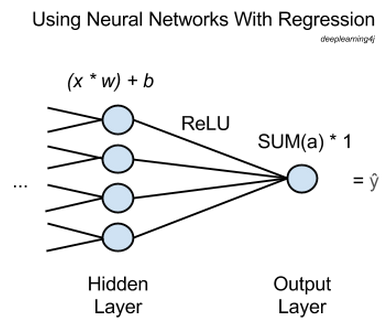
\includegraphics[width=0.4\linewidth]{neural-network-regression.png}
\caption{Neural Network}
\label{fig:neural_network}
\end{figure}

\section{Deep Learning}

Deep learning refers to artificial neural networks that are composed of many layers. Earlier 40 years back, neural networks were only 2 layers deep as it was not computationally feasible to build larger networks. But, now with better computing parts like Faster CPU, Faster GPU, large storage, now large neural networks are feasible.

And to accelerate the computing of these multi-layer neural networks, \textbf{ASIC}'s(Application specific Integrated Circuits) have been developed like \textbf{TPU}(Tensor Processing Units), which are designed to compute vector multiplications and additions.(AI accelerators)

\section{Parameter Server Architecture}

In Parameter server architecture, a job comprises two disjoint sets of processes- stateless worker processes and stateful parameter server. In this model, workers perform the bulk of computations and fetch the data from the parameter server and computed data is sent back to the parameter.

\section{DistBelief}

DistBelief was predecessor to TensorFlow, was implemented in C++. DistBelief uses Parameter Server Architecture.

\begin{itemize}
\item DistBelief was not flexible - It was hard to implement new algorithms in DistBelief like Softmax classifier, RandomForest algorithms etc.
\item DistBelief doesn't scale down - it is developed to be deployed in a cluster and cannot be used on a single pc.
\end{itemize}

\section{TensorFlow}
TensorFlow is a machine learning system that operates at large scale and in hetrogenous environments. 
\begin{itemize}
\item It uses data flow graphs(dfg) to represent computation shared state and the operations as well.
\item Data is represented in the form of \textbf{Tensors}- multi dimensional arrays.
\item Nodes are stateful which do bulk of computations.
\item Defers the execution until the entire program is available so that TensorFlow can optimize the execution phase by using global information about the computation.
\item Constant folding and common sub expression elimination are few of the optimizations that TensorFlow can perform.
\item TensorFlow represents the data/matrices in the form of the dense matrices only.(No support for sparse matrices)
\end{itemize}
\subsection{Dynamic Control Flow - Switch and Merge}

TensorFlow implements \textit{Switch} and \textit{Merge} primitives, which are borrowed from classic dynamic data flow architectures.

\begin{itemize}
\item Switch : is a demultiplexer. It takes a input data and a control input, and uses the control input to route the input data to one of its two outputs. The Switch utput not taken receives a special dead value, which propagates through the rest of graph until it reaches a Merge Operation.
\item Merge : is multiplexer. It forwards atmost one non-dead input to its output or if two inputs are dead values, then it produces a dead output. 
\end{itemize} 

\subsection{Operators - Variadic and Polymorphic}

\begin{itemize}
\item Polymorphic : Polymorphic mean that the operators in TensorFlow can operate on multiple types of data.
For example, a single Add operator can add Ints, Floats or Vectors of values.(Like Java generic functions)

\item Variadic : Variadic mean that the operators in TensorFlow can operate on different number of arguments.
For example, a single Add operator can add 2 variables or 3 variables etc.
\end{itemize}

\subsection{Stateful operations : Queue}

Queues(stores Tensors) allows concurrent access to tensors in the respective orders. These queue can block if the queue is full, thus providing backpressure and also supports synchronization ensuring deterministic results.

\end{document}

